\section{Application Processes}
\label{chap:improvement:application}

\mnote{Definition process}
The application of the \commonalities approach requires a process for defining them as well a concept for combining them with other specifications of transformations.
In a specification using the \commonalities approach, the \conceptmetamodels and manifestation relations are not as independent as they are supposed to be in the definition of an ordinary transformation network forming a dense or even complete graph.
Due to the necessity to relate all elements only via one transformation path, even if \commonalities are separated into \conceptmetamodels by concerns and composed hierarchically, the developers must ensure that such a structure is achieved.
We thus subsequently discuss different options how \commonalities can be defined.

\mnote{Combination concept}
We have identified in \autoref{chap:improvement:concepts:specification} that the \commonalities approach is well-suited for structural and \enquote{natural} consistency relations, rather than arbitrarily complex, in particular behavioral dependencies.
%This especially involves structural rather than behavioral consistency relations.
In the following, we discuss options for combining a \commonalities specification with other specifications, in particular ordinary transformations.


\subsection{Defining \Commonalities}

\mnote{Hierarchic composition}
We have discussed in \autoref{chap:improvement:commonalities:composition} how \commonalities and the \conceptmetamodels encapsulating them can be composed hierarchically.
This allows to separate \commonalities by concerns, i.e., by the concepts they belong to.
In addition, it fosters the independent development and reuse of different \conceptmetamodels.

\mnote{Independent development vs. tree structure}
The \commonalities approach does, however, only provide an essential benefit regarding guaranteed correctness of the resulting transformation network if the manifestation relations specify consistency relations that form a consistency relation tree (see \autoref{chap:improvement:commonalities:tree}).
Thus, \commonalities and their \conceptmetamodels must be composed in a way that such a structure is achieved.
This can, in the worst case, require all \concretemetamodels to define consistency between and the according relations to be elicited a priori and thus conflict with our independent development assumption.

\mnote{Bottom-up specification}
An intuitive process to define \commonalities is a bottom-up approach.
Developers select \concretemetamodels that share common concepts and are, by custom definition, most related among the \concretemetamodels to define consistency between and define a \conceptmetamodel of \commonalities between them.
Then, they iteratively choose \conceptmetamodels, and potentially also \concretemetamodels, that share further higher-level commonalities and define an according \conceptmetamodel for them.
This ends up in a hierarchy of \conceptmetamodels.

\mnote{Driven by \concretemetamodels}
Since finally instances of the \concretemetamodels are to be kept consistent, it is important to always consider the information represented in the \concretemetamodels, even if consistency is defined between \conceptmetamodels, i.e., at a higher level in the hierarchy of \conceptmetamodels.
Consider the running example of classes in \gls{UML} and Java, as well as components in \gls{UML}.
We may define an object-oriented design \conceptmetamodel to define \commonalities between \gls{UML} and Java, as well as a component-based design \conceptmetamodel to define \commonalities between object-oriented design and \gls{PCM}, as sketched in \autoref{chap:improvement:commonalities:tree} and depicted in \autoref{fig:improvement:composed_commonalities_example}.
If these \conceptmetamodels are defined in a bottom-up manner, i.e., first defining the object-oriented design \conceptmetamodel and afterwards the component-based design \conceptmetamodels, it is not sufficient to only consider the information represented in the object-oriented design \conceptmetamodels for defining their \commonalities.
That metamodel does only contain the \commonalities that are relevant for object-oriented design, but for the relation to component-based design, further information that is only present in one of the \concretemetamodels may be relevant.
For example, Java contains a definition of behavior in terms of method bodies, which is not represented in the purely structural \gls{UML} class models.
Thus, the object-oriented design \conceptmetamodel does not represent this behavioral information, as it does represent a \commonality.
\gls{PCM}, however, also has an abstract representation of behavior used for predicting the system's performance, which needs to be kept consistent with the precise behavior specification in Java.
Thus, the component-based design \conceptmetamodel must either have an additional manifestation relation to Java for the behavioral information, or the object-oriented design \conceptmetamodel must also contain behavioral information, although not being a \commonality between the \concretemetamodels it represents.

\mnote{Union of all information}
In general, this problem occurs because \conceptmetamodels are supposed to represent the unions of all pairwise intersections of their \concretemetamodels, as those represent the \commonalities that have to be kept consistent.
Information that is unique to one of the \concretemetamodels is not represented in the \conceptmetamodel, but may be relevant for further concepts and thus the relations to define to them.
A first, general solution would require a \conceptmetamodel to contain the union of all information in the \concretemetamodels rather than the union of their pairwise intersections.
This does, however, not conform to the purpose of \conceptmetamodels to only describe \commonalities.
It leads to large and complex \conceptmetamodels and thus also to high effort, because for each \concretemetamodel a transformation, in terms of a manifestation relation, of all its information to a \conceptmetamodel would have to be defined.
In addition, the topmost \conceptmetamodel of the hierarchy would inherently contain the union of information defined in all \concretemetamodels, thus representing a \gls{SUMM}, i.e., a single metamodel that is capable of representing all information to define one system (see \autoref{chap:foundations:multiview}). %, as introduced in \autoref{chap:improvement:concepts:explicit}.
In consequence, it would be sufficient to only manage an instance of that topmost \conceptmetamodel, representing the \gls{SUMM}, and to consider the instances of all other concept and \concretemetamodels as projections from the instance of that central metamodel, according to \textcite{atkinson2010a}.

\begin{figure}
    \centering
    \newcommand{\vdistance}{8em}
\newcommand{\hdistance}{14em}
\newcommand{\classwidth}{5.5em}
\newcommand{\labeldistance}{1em}
\newcommand{\labelshift}{0.3*\classwidth}
\newcommand{\mmborder}{1em}

\begin{tikzpicture}

\pgfdeclarelayer{bg}
\pgfsetlayers{bg,main}


% METACLASSES

\umlclassvarwidth{java_class}{}{Class}{
name\\
visbility\\
** behavior **
}{\classwidth}

\umlclassvarwidth[, right=0.8*\hdistance of java_class.north, anchor=north]{uml_class}{}{Class}{
name\\
visbility\\
}{\classwidth} 

\umlclassvarwidth[, above right=1.1*\vdistance and 0.5*\hdistance of java_class.north, anchor=north]{oo_class}{}{Class\vphantom{p}}{
name\\
visibility\\
** behavior **
}{\classwidth} 

\umlclassvarwidth[, right=\hdistance of oo_class.north, anchor=north]{pcm_component}{}{Component}{
name\\
** behavior **
}{\classwidth} 

\umlclassvarwidth[, above right=1.1*\vdistance and 0.5*\hdistance of oo_class.north, anchor=north]{component_component}{}{Component}{
name\\
visbility\\
** behavior **
}{\classwidth}

% METAMODELS

\coordinate (java_label_coordinate) at ([yshift=\labeldistance]java_class.north west);
\node[mmlabel, anchor=west] (java_label) at (java_label_coordinate) {Java};

\coordinate (uml_label_coordinate) at ([yshift=\labeldistance]uml_class.north east);
\node[mmlabel, anchor=east] (uml_label) at (uml_label_coordinate) {\acrshort{UML}};

\coordinate (oo_label_coordinate) at ([xshift=-4*\labelshift,yshift=\labeldistance]oo_class.north);
\node[mmlabel, anchor=west, align=left] (oo_label) at ([xshift=-0.5em, yshift=-0.7em]oo_label_coordinate) {Object-oriented\\ Design};

\coordinate (pcm_label_coordinate) at ([yshift=\labeldistance]pcm_component.north east);
\node[mmlabel, anchor=east] (pcm_label) at (pcm_label_coordinate) {\acrshort{PCM}};

\coordinate (component_label_coordinate) at ([yshift=\labeldistance]component_component.north);
\node[mmlabel, anchor=center] (component_label) at (component_label_coordinate) {Component-based Design};

\begin{pgfonlayer}{bg}
    \node[mmbg, fit=(java_class)(java_label.west), inner sep=\mmborder] (java) {};
    \node[mmbg, fit=(uml_class)(uml_label.east), inner sep=\mmborder] (uml) {};
    \node[conceptmmbg, fit=(oo_class)(oo_label_coordinate), inner sep=\mmborder] (oo) {};
    \node[mmbg, fit=(pcm_component)(pcm_label.east), inner sep=\mmborder] (pcm) {};
    \node[conceptmmbg, fit=(component_component)(component_label.west)(component_label.east), inner sep=\mmborder] (component) {};
\end{pgfonlayer}


% CONSISTENCY RELATIONS

\draw[manifests relation] (oo_class) -- node[manifests relation, above, sloped] {\manifestslabel} (java_class);
\draw[manifests relation] (oo_class) -- node[manifests relation, above, sloped] {\manifestslabel} (uml_class);
\draw[manifests relation] (component_component) -- node[manifests relation, above, sloped] {\manifestslabel} (oo_class);
\draw[manifests relation] (component_component) -- node[manifests relation, above, sloped] {\manifestslabel} (pcm_component);

\end{tikzpicture}

    \caption[\Commonalities with union of all information]{Example for a hierarchy of \conceptmetamodels and their \commonalities in which \conceptmetamodels represent the union of information in their manifestations. Behavior of classes and components is considered any, not further specified kind of behavioral information.}
    \label{fig:improvement:definition_option_sum}
\end{figure}

\mnote{Example for union}
For the example int \autoref{fig:improvement:composed_commonalities_example} depicting hierarchic \conceptmetamodels for classes and components, we derive an extension according to the discussed scheme in \autoref{fig:improvement:definition_option_sum}.
It additionally contains visibilities for classes and any kind of not further specified behavior description in Java classes and \gls{PCM} components.
Both \conceptmetamodels contain the union information in their manifestations, such that the component-based design \conceptmetamodel contains all information represented in all metamodels.
In consequence, the component-based design \conceptmetamodel represents the visibility of classes in object-oriented design, although it is not relevant for components and is not kept consistent via that \conceptmetamodel.

\mnote{Non-strict manifestations}
The previous considerations assume a kind of strict layered architecture (see~\cite{buschmann1996PatternsArchitecture-Book}) in which the manifestation relations induce a tree between the metamodels, thus no manifestation relation bypasses a \conceptmetamodel to whose \commonalities additional manifestation relations are defined.
Referring to a non-strict layered architecture, another solution would be to allow manifestation relations to the manifestations of \conceptmetamodels to which further manifestation relations are defined, e.g., the component-based design \commonalities may have manifestation relations to elements in Java and \gls{UML} in addition to manifestation relations to the object-oriented design \conceptmetamodels, which in turn has manifestation relations to those \concretemetamodels.
A drawback of this solution is that it can likely violate the goal of achieving a tree structure.
Considering a class in Java as a manifestation of a component in component-based design, as well as a class in object-oriented design, which in turn is a manifestation of a component in component-based design, would already violate the definition of a consistency relation tree, thus not giving guarantees regarding compatibility.

\begin{figure}
    \centering
    \newcommand{\vdistance}{8em}
\newcommand{\hdistance}{14em}
\newcommand{\classwidth}{5.5em}
\newcommand{\labeldistance}{1em}
\newcommand{\labelshift}{0.3*\classwidth}
\newcommand{\mmborder}{1em}

\begin{tikzpicture}

\pgfdeclarelayer{bg}
\pgfsetlayers{bg,main}


% METACLASSES

\umlclassvarwidth{java_class}{}{Class}{
name\\
visbility\\
** behavior **
}{\classwidth}

\umlclassvarwidth[, right=0.8*\hdistance of java_class.north, anchor=north]{uml_class}{}{Class}{
name\\
visbility\\
}{\classwidth} 

\umlclassvarwidth[, above right=\vdistance and 0.5*\hdistance of java_class.north, anchor=north]{oo_class}{}{Class\vphantom{p}}{
name\\
visibility\\
}{\classwidth} 

\umlclassvarwidth[, right=\hdistance of oo_class.north, anchor=north]{pcm_component}{}{Component}{
name\\
** behavior **
}{\classwidth} 

\umlclassvarwidth[, above right=\vdistance and 0.5*\hdistance of oo_class.north, anchor=north]{component_component}{}{Component}{
name\\
** behavior **
}{\classwidth}

% METAMODELS

\coordinate (java_label_coordinate) at ([yshift=\labeldistance]java_class.north west);
\node[mmlabel, anchor=west] (java_label) at (java_label_coordinate) {Java};

\coordinate (uml_label_coordinate) at ([yshift=\labeldistance]uml_class.north east);
\node[mmlabel, anchor=east] (uml_label) at (uml_label_coordinate) {\acrshort{UML}};

\coordinate (oo_label_coordinate) at ([xshift=-4*\labelshift,yshift=\labeldistance]oo_class.north);
\node[mmlabel, anchor=west, align=left] (oo_label) at ([xshift=-0.5em, yshift=-0.7em]oo_label_coordinate) {Object-oriented\\ Design};

\coordinate (pcm_label_coordinate) at ([yshift=\labeldistance]pcm_component.north east);
\node[mmlabel, anchor=east] (pcm_label) at (pcm_label_coordinate) {\acrshort{PCM}};

\coordinate (component_label_coordinate) at ([yshift=\labeldistance]component_component.north);
\node[mmlabel, anchor=center] (component_label) at (component_label_coordinate) {Component-based Design};

\begin{pgfonlayer}{bg}
    \node[mmbg, fit=(java_class)(java_label.west), inner sep=\mmborder] (java) {};
    \node[mmbg, fit=(uml_class)(uml_label.east), inner sep=\mmborder] (uml) {};
    \node[conceptmmbg, fit=(oo_class)(oo_label_coordinate), inner sep=\mmborder] (oo) {};
    \node[mmbg, fit=(pcm_component)(pcm_label.east), inner sep=\mmborder] (pcm) {};
    \node[conceptmmbg, fit=(component_component)(component_label.west)(component_label.east), inner sep=\mmborder] (component) {};
\end{pgfonlayer}


% CONSISTENCY RELATIONS

\draw[manifests relation] (oo_class) -- node[stereotype, above, sloped] {\manifestslabel} (java_class);
\draw[manifests relation] (oo_class) -- node[stereotype, above, sloped] {\manifestslabel} (uml_class);
\draw[manifests relation] (component_component) -- node[stereotype, above, sloped] {\manifestslabel} (oo_class);
\draw[manifests relation] (component_component) -- node[stereotype, above, sloped] {\manifestslabel} (pcm_component);
\draw[manifests relation] (component_component) .. controls ([yshift=-0.5em,xshift=-\hdistance]component_component.west) and ([yshift=2*\vdistance]java_class.north west) .. ([xshift=-0.5em]java_class.north) node[stereotype, pos=0.25, above] {\manifestslabel};

\end{tikzpicture}

    \caption[\Commonalities with multiple manifestation]{Example for a hierarchy of \conceptmetamodels and their \commonalities, in which \commonalities may have several manifestations inducing consistency relations that do not form a tree structure. Behavior of classes and components is considered any, not further specified kind of behavioral information.}
    \label{fig:improvement:definition_option_bypass}
\end{figure}

\mnote{Example for non-strict manifestations}
\autoref{fig:improvement:definition_option_bypass} depicts this solution for the already discussed example.
The \conceptmetamodels contain only the information relevant for the \commonalities they represent.
The additional manifestation relation between components of the component-based design \conceptmetamodel and classes in Java induce the violation of a tree structure as sketched before.
Although behavior may actually be represented in terms of method bodies represented as separate \metaclasses in Java, still consistency relations defined by the manifestation relations between Java and the object-oriented design \conceptmetamodel would include both classes and methods, as methods do not share an isolated consistency relation between Java and \gls{UML} but only in the context of the class they belong to.

\mnote{Union including concepts}
A third option is to construct a \conceptmetamodel not only driven by the \commonalities shared between its manifestations, but also by its \commonalities with other metamodels.
Thus, whenever a \conceptmetamodel is used as a manifestation of another \conceptmetamodel, it may be extended by the information from its manifestations required for the \commonalities in another concept with other metamodels.
For example, as soon as the object-oriented design \conceptmetamodel is considered as a manifestation of component-based design, its manifestations, namely Java and \gls{UML}, are checked for \commonalities with component-based design that are not yet considered \commonalities regarding object-oriented design.
This could be a description of method bodies in Java to keep consistent with the behavior specification in \gls{PCM}.
If consequently followed, such an approach would result in \conceptmetamodels not only representing the union of the pairwise intersections of the manifestations, but the union of the pairwise intersections of their manifestations with all other \concretemetamodels to be kept consistent.
This still promises to lead to \conceptmetamodels that are significantly smaller and more precise than the union of all metamodels as in the first option, but still allow to achieve a tree structure, which is why we propose to use this option.
This approach is comparable to the situation in which a further manifestation shall be added, like we exemplarily discussed for adding \cplusplus as a manifestation of the object-oriented design \conceptmetamodel in \autoref{chap:improvement:benefits:specification_effort}.

\begin{figure}
    \centering
    \newcommand{\vdistance}{7.7em}
\newcommand{\hdistance}{14em}
\newcommand{\classwidth}{5.5em}
\newcommand{\labeldistance}{1em}
\newcommand{\labelshift}{0.3*\classwidth}
\newcommand{\mmborder}{1em}

\begin{tikzpicture}

\pgfdeclarelayer{bg}
\pgfsetlayers{bg,main}


% METACLASSES

\umlclassvarwidth{java_class}{}{Class}{
name\\
visbility\\
** behavior **
}{\classwidth}

\umlclassvarwidth[, right=0.8*\hdistance of java_class.north, anchor=north]{uml_class}{}{Class}{
name\\
visbility\\
}{\classwidth} 

\umlclassvarwidth[, above right=1.2*\vdistance and 0.5*\hdistance of java_class.north, anchor=north]{oo_class}{}{Class\vphantom{p}}{
name\\
visibility\\
** behavior **
}{\classwidth} 

\umlclassvarwidth[, right=\hdistance of oo_class.north, anchor=north]{pcm_component}{}{Component}{
name\\
** behavior **
}{\classwidth} 

\umlclassvarwidth[, above right=\vdistance and 0.5*\hdistance of oo_class.north, anchor=north]{component_component}{}{Component}{
name\\
** behavior **
}{\classwidth}

% METAMODELS

\coordinate (java_label_coordinate) at ([yshift=\labeldistance]java_class.north west);
\node[mmlabel, anchor=west] (java_label) at (java_label_coordinate) {Java};

\coordinate (uml_label_coordinate) at ([yshift=\labeldistance]uml_class.north east);
\node[mmlabel, anchor=east] (uml_label) at (uml_label_coordinate) {UML};

\coordinate (oo_label_coordinate) at ([xshift=-4*\labelshift,yshift=\labeldistance]oo_class.north);
\node[mmlabel, anchor=west, align=left] (oo_label) at ([xshift=-0.5em, yshift=-0.7em]oo_label_coordinate) {Object-oriented\\ Design};

\coordinate (pcm_label_coordinate) at ([yshift=\labeldistance]pcm_component.north east);
\node[mmlabel, anchor=east] (pcm_label) at (pcm_label_coordinate) {PCM};

\coordinate (component_label_coordinate) at ([yshift=\labeldistance]component_component.north);
\node[mmlabel, anchor=center] (component_label) at (component_label_coordinate) {Component-based Design};

\begin{pgfonlayer}{bg}
    \node[mmbg, fit=(java_class)(java_label.west), inner sep=\mmborder] (java) {};
    \node[mmbg, fit=(uml_class)(uml_label.east), inner sep=\mmborder] (uml) {};
    \node[conceptmmbg, fit=(oo_class)(oo_label_coordinate), inner sep=\mmborder] (oo) {};
    \node[mmbg, fit=(pcm_component)(pcm_label.east), inner sep=\mmborder] (pcm) {};
    \node[conceptmmbg, fit=(component_component)(component_label.west)(component_label.east), inner sep=\mmborder] (component) {};
\end{pgfonlayer}


% CONSISTENCY RELATIONS

\draw[manifests relation] (oo_class) -- node[manifests relation, above, sloped] {\manifestslabel} (java_class);
\draw[manifests relation] (oo_class) -- node[manifests relation, above, sloped] {\manifestslabel} (uml_class);
\draw[manifests relation] (component_component) -- node[manifests relation, above, sloped] {\manifestslabel} (oo_class);
\draw[manifests relation] (component_component) -- node[manifests relation, above, sloped] {\manifestslabel} (pcm_component);

\end{tikzpicture}

    \caption[\Commonalities including information of their concepts]{Example for a hierarchy of \conceptmetamodels and their \commonalities, in which \commonalities represent information necessary for the concepts they are manifestations of in addition to the information shared by their manifestations. Behavior of classes and components is considered any, not further specified kind of behavioral information.}
    \label{fig:improvement:definition_option_super_union}
\end{figure}

\mnote{Example for union including concepts}
The application of this option to the already discussed example is depicted in \autoref{fig:improvement:definition_option_super_union}.
In this solution, still a tree structure between the \metaclasses and \commonalities is given and the \conceptmetamodels are still restricted to the information in the manifestations and, in addition, the information of the manifestations necessary for the \conceptmetamodels of which they are manifestations.
This is why the object-oriented design \conceptmetamodel contains information about the behavior of classes and components, although \gls{UML} and Java do not share behavioral concepts, but the component \commonality for component-based design does not contain the visibilities of classes as in the first option of representing the union of all information in the manifestations.

\mnote{Problem mitigation by cliques}
Finally, it is still an open question how problematic the actual dependencies in practical scenarios are.
Potentially, only subsets of few metamodels are highly related and share large parts of one or more concepts, and the relation to other such subsets is only given across one metamodel or one concept.
This could be seen as a graph of cliques, in which some metamodels are highly related whereas the relation to others is rather loose.
In that case, it can be reasonable to define relations in these cliques by means of \commonalities and then define the loose relations to other cliques by means of an ordinary transformation, as we discuss in the subsequent section.
We derive first insights on the achievability of the required tree structure for \commonalities in our evaluation in \autoref{chap:commonalities_evaluation}, but further evidence if one of the previously discussed strategies can be reasonably applied has to be gained in larger studies in practical scenarios with more metamodels of more tools.

% Discuss how commonalities can be defined. Which roles are involved, especially how different domain experts can communicate. E.g., bottom-up approach: Take the most related metamodels and define their commonalities. Then define higher-level commonalities relating these concept metamodels or even the concrete metamodels. 
% The problem is that combining two concept metamodels requires them to contain all necessary information, thus a concept metamodel design is not only driven by the metamodels to keep directly consistent, but also by the information that is needed to preserve consistency to other commonalities. This refers to the same scenario as if multiple commonality structures are encapsulated into projective view environments which are combined by BX. They require the exposed views to provide all information necessary to preserve consistency.

% Prozess zur Erzeugung von Commonalities beschreiben:
% - Optimalerweise kennt man alle MM vorher und kann sinnvolle Commonalities bauen (immer das am wenigstens redundante Konstrukt, z.B. eher Person in Familie als Persons mit Familiennamen (redundante Darstellung des Familiennamens)
% - Bei Erweiterung um zusätzliche Metamodelle sind ggf. Anpassungen an Commonalities notwendig. Hier ist wieder die Lokalität bei den Commonalities vorteilhaft (interne Spezifikation), weil man dann eine Commonality insgesamt ersetzen kann statt in jeder Transformation deren Manifestierung anzupassen.

% Evolutionsprozess:
% - Wie eignet sich welcher Ansatz zur Erweiterung mit MM. I.d.R. reicht es nicht eine Verbindung zu ergänzen, sondern die Konzeptmetamodelle für angepasst werden für ein neuen zu koppelndes Metamodell


\subsection{Combining \Commonalities}

\mnote{Necessity for combination}
We have up to now discussed how to construct \conceptmetamodels and manifestation relations in terms of the \commonalities approach, such that the topology of the defined relations fulfills the definition of a consistency relation tree to achieve inherent guarantees regarding correctness of the transformation network.
We have also derived how the \commonalities approach improves reusability in comparison to the construction of a transformation network with tree topology out of the \concretemetamodels.
Nevertheless, the approach has at least two limitations, which we have already identified.
First, it lacks completeness, as it requires a specific topology of consistency relations to be achievable, which is likely to get more complex the more metamodels are involved.
Second, it only fits well for structural relations in which actual commonalities can be described or prescribed.

\mnote{\Commonalities for subsets}
In consequence, to improve applicability of the approach, it should be applied for subsets of metamodels that inherently share commonalities, comparable to the cliques mentioned before, which are suited to be described with the proposed approach.
These specifications should then be combined with other consistency specifications, be they defined with the \commonalities approach or with ordinary transformations.
Such a combination would restrict the size and complexity of a hierarchy of \commonalities and could foster reuse of consistency specifications for specific concepts in different context, as motivated by our assumptions of independent development and modular reuse, as well as the process proposed in \autoref{chap:networks:specification_process}.

\begin{figure}
    \centering
    \newcommand{\mmdistance}{8em}

\begin{tikzpicture}[
    mm/.style={schematic metamodel},
    conceptmm/.style={schematic conceptmetamodel}
]

\node[mm] (original_left) {$\metamodel{A}{}$};
\node[mm, right=\mmdistance of original_left.center, anchor=center] (original_middle) {$\metamodel{B}{}$};
\node[mm, right=\mmdistance of original_middle.center, anchor=center] (original_right) {$\metamodel{C}{}$};
\node[conceptmm, above right=0.8*\mmdistance and 0.5*\mmdistance of original_left.center, anchor=center, align=center] (concept) {$\metamodel{AB}{\mathvariable{Concepts}}$};

\draw[consistency relation] (original_left) -- node[above] {$\consistencyrelation{CR}{AB}$} (original_middle);
\draw[consistency relation] (original_middle) to[bend left=30] node[above] {$\consistencyrelation{CR}{BC}$} (original_right);
\draw[consistency relation] (original_left) to[bend right=35] node[above] {$\consistencyrelation{CR}{AC}$} (original_right);

\draw[consistency relation, color=gray] (original_left) -- node[above left=-0.3em and 0.5em] {$\consistencyrelation{CR}{A}$} (concept);
\draw[consistency relation, color=gray] (original_middle) -- node[above right=-0.3em and 0.3em] {$\consistencyrelation{CR}{B}$} (concept);
\draw[consistency relation, color=gray] (original_right) to[bend right=30] node[pos=0.6, below left] {$\consistencyrelation{CR}{C}$} (concept);


\node[right=3*\mmdistance+0.4*\difftoafiveimage of concept.north, anchor=north east, align=left] (constraints_top) { 
$\consistencyrelation{CR}{AB} \concat \consistencyrelation{CR}{BC} \neq (\consistencyrelation{CR}{AB} \concat \consistencyrelation{CR}{BC}) \cap \consistencyrelation{CR}{AC} \neq \consistencyrelation{CR}{AC}$
};

\node[below=2em of constraints_top.north east, anchor=north east, align=left] {
$\consistencyrelation{CR}{A} \concat \consistencyrelation{CR}{B} = \consistencyrelation{CR}{AB}$\\
$\consistencyrelation{CR}{A} \concat \consistencyrelation{CR}{C} = \consistencyrelation{CR}{AC}$\\
$\consistencyrelation{CR}{B} \concat \consistencyrelation{CR}{C} = \consistencyrelation{CR}{BC}$\\
};

\end{tikzpicture}
    \caption[Partial transformation network of \commonalities]{Example for a \conceptmetamodel to replace a consistency relation and the replacement of ordinary consistency relations to the \concretemetamodels with one to the \conceptmetamodel. Adapted from~\owncite[Fig.~5]{klare2018docsym}.}
    \label{fig:improvement:commonalities_combination_generic}
\end{figure}

\mnote{General combination requirements}
To preserve the benefits of a \commonalities specification, it can be combined with other specifications, be they ordinary transformations or another \commonalities specification, by considering any of the other metamodels as a manifestation or a \conceptmetamodel of one of the \conceptmetamodels of the \commonalities specifications.
This preserves the tree structures of the \commonalities specification and its benefits.
Consider the generic example in \autoref{fig:improvement:commonalities_combination_generic} with three metamodels, a \conceptmetamodel for two of them and consistency relations between them, which are considered \modellevelconsistencyrelations according to \autoref{def:modellevelconsistencyrelation} for reasons of simplicity.
The consistency relation $\consistencyrelation{CR}{AB}$ between metamodels $\metamodel{A}{}$ and $\metamodel{B}{}$ is expressed by a \conceptmetamodel $\metamodel{AB}{\mathvariable{Concepts}}$ and consistency relations for the according manifestation relations $\consistencyrelation{CR}{A}$ and $\consistencyrelation{CR}{B}$.
In addition, the metamodel $\metamodel{C}{}$ shares consistency relations with both other metamodels.
To preserve reusability and the necessary tree structure, these consistency relations $\consistencyrelation{CR}{AB}$ and $\consistencyrelation{CR}{AC}$ should be described in terms of a consistency relation $\consistencyrelation{CR}{C}$ to the concept metamodel.
This does, however, require the \conceptmetamodel to contain all information that is necessary to preserve consistency between $\metamodel{C}{}$ and the two others, as described with the required relations in \autoref{fig:improvement:commonalities_combination_generic}.
In contrast to the scenarios discussed in the previous section for how to define \conceptmetamodels and which information to put into them, if $\metamodel{C}{}$ is a part of a different consistency specification to combine the \commonalities specification with, or if the \commonalities specification covers more than two \concretemetamodels with one \conceptmetamodel, this can require an arbitrarily complex adaptation, which may even not be wanted of possible at all if modular reuse is desired.

\mnote{Virtualization by views}
To improve such a combination of specifications, virtualization concepts as known from \gls{OSM}~\cite{atkinson2010a} (see \autoref{chap:foundations:multiview:osm}) and the \vitruv approach~\cite{klare2020Vitruv-JSS} (see \autoref{chap:foundations:multiview:vitruv}) can be applied.
Their idea is to encapsulate metamodels and their instances behind a facet of views and to enable access to the actual models only via these views.
Views are projections of the encapsulated models, i.e., they derive all information from the models and potentially aggregate them or arrange them differently.
The metamodels of these views are called \emph{\viewtypes}.
While those approaches were originally designed to provide a well-defined interface through views for developers and internally ensure consistency of the persisted artifacts by either avoiding or managing redundancy, they can also be used as an interface for consistency preservation.
In the \vitruv approach, a so called \gls{VSUM} is composed of models and rules for preserving their consistency, whose contents are exposed by views to be modified by developers.

\begin{figure}
    \centering
    % requires tikzvitruvius.sty
\begin{tikzpicture}[
    vtcaption/.style={font=\small},
    view/.style={uml box, densely dashed},
    viewtype/.style={circle, draw, solid, fill=white, inner sep=.1em, font=\scriptsize},
    polarrow/.style={latex-latex, densely dotted},
    mininode/.style={inner sep=.4em},
    uniformly sized package/.style={minimum width=2.5em},
]

% V-SUM
\umlpackage[uniformly sized package]{oo}{}{OOD}
\umlpackage[uniformly sized package]{uml}{below left=4.5em and 0em of oo}{\acrshort{UML}}
\umlpackage[uniformly sized package]{java}{below right=4.5em and 0em of oo}{Java}

\node[circle,draw,thick,fit=(oo.center)(uml)(java),inner sep=2ex] (sum) {};

\draw[manifests relation] (oo) -- node[manifests relation, above, sloped] (pcmJavaCCR) {\manifestslabel} (uml.north);
\draw[manifests relation] (oo) -- node[manifests relation, above, sloped] (pcmJavaCCR) {\manifestslabel} (java.north);

\node[viewtype] (viewtypeOO) at (sum.60) {$\mathvariable{VT}_\mathvariable{OOD}$};
\node[viewtype] (viewtypeJava) at (sum.5) {$\mathvariable{VT}_\mathvariable{Java}$};
\draw[polarrow] (oo) -- (viewtypeOO);
\draw[polarrow] (java) -- (viewtypeJava);

\node[font=\bfseries\footnotesize] (sumtext) [above=0.6em of sum.270, anchor=south, align=center] {\vsum\\ Metamodel};

% Outer transformations
\umlpackage[uniformly sized package]{pcm}{above right=-0.5em and 13em of oo}{\acrshort{PCM}};
\draw[transformation] (viewtypeOO) -- node[transformation, above, sloped] {Structure} (pcm);
\draw[transformation] (viewtypeJava) -- node[transformation, above, sloped] {Behavior} (pcm);

% Legend
\node[draw, legendbg, matrix, font=\scriptsize, inner sep=0.7em, nodes=mininode] (legend) at (17.5em,-5.8em) {%
    \umlpackage[minimum height=0.1em, inner sep=0.3em, yshift=0.5ex, font=\scriptsize, xshift=1.25em]{legend_mm}{}{MM} & \node[anchor=base west, font=\footnotesize] {Metamodel\sameheight};\\
    \node[viewtype, xshift=1.25em, yshift=0.5ex, font=\scriptsize] {$\mathvariable{VT}$}; & \node[anchor=base west, font=\footnotesize] {\ViewType\sameheight};\\
    \draw[polarrow] (0,.5ex)--(2.5em,.5ex); & \node[anchor=base west, font=\footnotesize] {View Transformation\sameheight};\\
    \draw[transformation] (0,.5ex)--(2.5em,.5ex); & \node[anchor=base west, font=\footnotesize] {Transformation\sameheight};\\
};

\end{tikzpicture}

    %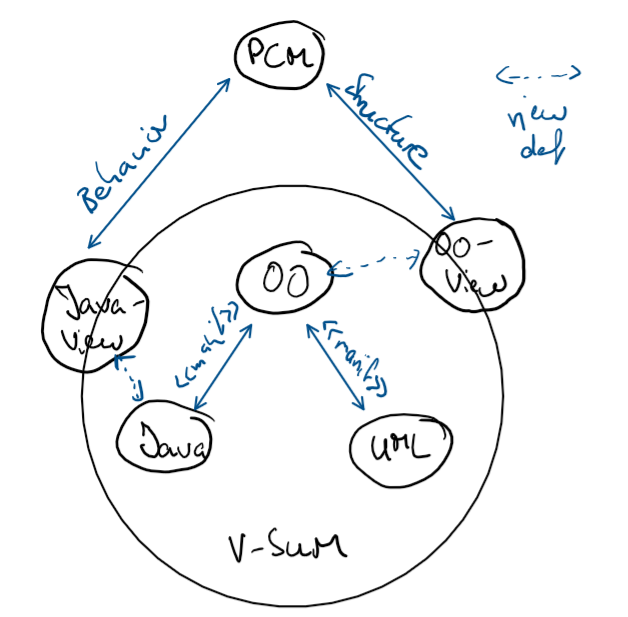
\includegraphics[width=0.6\textwidth]{figures/quality/improvement/combination_external_metamodel.png}
    \caption[Combination of \commonalities with a transformation]{Example for the combination of a \commonalities specification for object-oriented design (OOD) with \gls{PCM} by encapsulation into a \vsumm.}
    \label{fig:improvement:combination_external_metamodel}
\end{figure}

\mnote{Encapsulation of \commonalities in \vsum}
Consider the example depicted in \autoref{fig:improvement:combination_external_metamodel}.
It comprises the \commonalities specification for Java and \gls{UML} using a single \conceptmetamodel for object-oriented design.
This consistency specification by means of \commonalities is encapsulated into a \vsum, which exposes the Java code via a Java view and the object-oriented structure represented in instances of the \conceptmetamodel as an object-oriented view.
These two views are then related to \gls{PCM} by means of ordinary consistency relations and transformations preserving them.
The relations between metamodels and \viewtypes can, again, be considered ordinary transformations.
Thus, the defined transformation network would actually contain cycles, such that it does not benefit from the \commonalities specification within the \vsum in terms of correctness.
If we do only consider the \vsum itself, it does, however, still have a tree structure, so if only one of the views is modified at the same time, it provides the benefits that we have discussed for a \commonalities specification in \autoref{chap:improvement:benefits}.
In addition, views of a \vsum by now actually assume that only one of them is changed at a time~\cite{klare2020Vitruv-JSS}, as a developer is supposed to work on one specific view at a time.
Thus, if the transformations outside the \vsum ensure that only one of the views is changed at a time, the \vsum provides the discussed benefits of the \commonalities approach.

\mnote{Clarification of responsibilities}
This approach does, of course, not solve possible issues regarding synchronization and orchestration in the transformation network defined outside the \vsum, but only moves the problem of avoiding these issues away from the \commonalities specification by making according assumptions in terms of allowing only modifications of one view of a \vsum.
It does, however, clarify responsibilities, as there are precisely defined views across which other metamodels can be combined with those for which consistency is defined by means of \commonalities, rather than defining consistency to the metamodels within the \commonalities specification directly and thus breaking the necessary assumption for the intended benefits of that approach.
In the example, we have a clear separation into views for the structure of the object-oriented representation in Java, \gls{UML} and potentially more metamodels, and for its behavior.
It is up to the developer of the transformation network outside the \vsum to ensure that no problems like execution loops occur by assigning clear non-conflicting responsibilities to the two transformations for structure and behavior of the \vsum to \gls{PCM}.

\begin{figure}
    \centering
    % requires tikzvitruvius.sty
\begin{tikzpicture}[
    vtcaption/.style={font=\small},
    view/.style={uml box, densely dashed},
    viewtype/.style={circle, draw, solid, fill=white, inner sep=.1em, font=\scriptsize},
    polarrow/.style={latex-latex, densely dotted},
    mininode/.style={inner sep=.4em},
    uniformly sized package/.style={minimum width=2.5em},
]

% V-SUM 1
\umlpackage[uniformly sized package]{oo}{}{OOD}
\umlpackage[uniformly sized package]{uml}{below left=4.5em and 0em of oo}{UML}
\umlpackage[uniformly sized package]{java}{below right=4.5em and 0em of oo}{Java}

\node[circle,draw,thick,fit=(oo.center)(uml)(java),inner sep=2ex] (sum1) {};

\draw[manifests relation] (oo) -- node[manifests relation, above, sloped] (pcmJavaCCR) {\manifestslabel} (uml.north);
\draw[manifests relation] (oo) -- node[manifests relation, above, sloped] (pcmJavaCCR) {\manifestslabel} (java.north);

\node[viewtype] (viewtypeOO) at (sum1.40) {$\mathvariable{VT}_\mathvariable{OOD}$};
\node[viewtype] (viewtypeJava) at (sum1.5) {$\mathvariable{VT}_\mathvariable{Java}$};
\draw[polarrow] (oo) -- (viewtypeOO);
\draw[polarrow] (java) -- (viewtypeJava);

\node[font=\bfseries\footnotesize] (sum1text) [above=0.6em of sum1.270, anchor=south, align=center] {\vsum\\ Metamodel};

% V-SUM 2
\umlpackage[uniformly sized package]{cbd}{right=14.8em of oo}{CBD}
\umlpackage[uniformly sized package]{pcm}{below left=4.5em and 0em of cbd}{PCM}
\umlpackage[uniformly sized package]{umlcomp}{below right=4.5em and 0em of cbd}{UML}

\node[circle,draw,thick,fit=(cbd.center)(pcm)(umlcomp),inner sep=2ex] (sum2) {};

\draw[manifests relation] (cbd) -- node[manifests relation, above, sloped] (pcmJavaCCR) {\manifestslabel} (pcm.north);
\draw[manifests relation] (cbd) -- node[manifests relation, above, sloped] (pcmJavaCCR) {\manifestslabel} (umlcomp.north);

\node[viewtype] (viewtypeStruc) at (sum2.140) {$\mathvariable{VT}_\mathvariable{Structure}$};
\node[viewtype] (viewtypeBehav) at (sum2.175) {$\mathvariable{VT}_\mathvariable{Behavior}$};
\draw[polarrow] (cbd) -- (viewtypeStruc);
\draw[polarrow] (pcm.north west) -- (viewtypeBehav);

\node[font=\bfseries\footnotesize] (sum2text) [above=0.6em of sum2.270, anchor=south, align=center] {\vsum\\ Metamodel};

% Outer transformations
\draw[transformation] (viewtypeOO) -- (viewtypeStruc);
\draw[transformation] (viewtypeJava) -- (viewtypeBehav);

\coordinate (middle) at ($(oo)!0.5!(cbd)$);

% Legend
\node[draw, legendbg, matrix, font=\scriptsize, inner sep=0.7em, nodes=mininode, anchor=north, below=10.5em of middle] (legend) {%
    \umlpackage[minimum height=0.1em, inner sep=0.3em, yshift=0.5ex, font=\scriptsize, anchor=center]{legend_mm}{}{MM} & \node[anchor=base west, font=\footnotesize] {Metamodel \hspace{0.5em}\sameheight}; &
    \draw[polarrow] (0em,0.5ex)--(2em,0.5ex); & \node[anchor=base west, font=\footnotesize] {View Transformation\sameheight}; \\
    \node[viewtype, anchor=center, yshift=0.5ex, font=\scriptsize] {$\mathvariable{VT}$}; & \node[anchor=base west, font=\footnotesize] {\ViewType\sameheight};&
    \draw[transformation] (0em,0.5ex)--(2em,0.5ex); & \node[anchor=base west, font=\footnotesize] {Transformation\sameheight};\\
};

\end{tikzpicture}

    %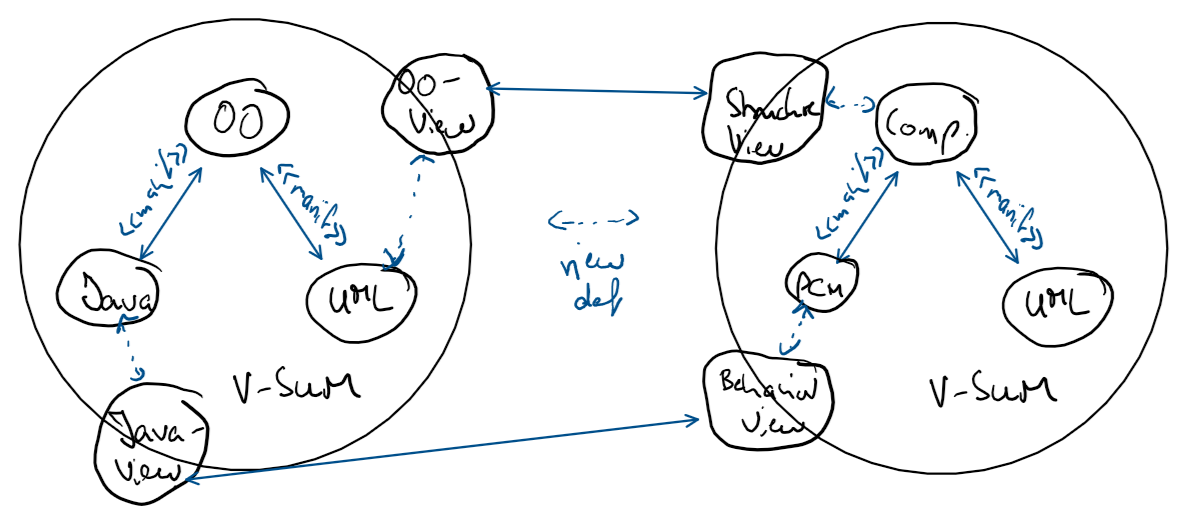
\includegraphics[width=\textwidth]{figures/quality/improvement/combination_two_vsums.png}
    \caption[Combination of two \commonalities specifications]{Example for the combination of two \commonalities specifications for object-oriented (OOD) and component-based design (CBD) by encapsulation into \vsumms.}
    \label{fig:improvement:combination_two_vsums}
\end{figure}

\mnote{Combination of encapsulating \vsums}
Instead of only \gls{PCM}, there could be a more complex transformation network, or another \commonalities specification, which may again be encapsulated into a \vsum and provide its own views, across which both \vsums can then be combined.
\autoref{fig:improvement:combination_two_vsums} depicts such an example, in which \gls{PCM} and \gls{UML} component models are related by a \conceptmetamodel for component-based design, encapsulated into a second \vsum.
This \vsum provides separate \viewtypes for the structure represented by both \gls{PCM} and \gls{UML} and thus reflected in the \conceptmetamodels, and for the behavior only represented in \gls{PCM}.
These \viewtypes can then be combined by means of ordinary transformations with those of the \vsum for object-oriented design.
Again, this approach does not prevent the occurrence of correctness issues as discussed in \autoref{part:correctness} due to the transformations outside the \vsum, but at least within each \vsum we can guarantee correctness.

\mnote{Hierachic composition of \vsums}
This approach can even be hierarchically be composed, such that several kinds of specifications, including encapsulating \vsums, are again encapsulated into another \vsum.
For example, the \vsums in \autoref{fig:improvement:combination_two_vsums} could be encapsulated into a \vsum for object-oriented and component-based design to be reused together.
If the transformation network between the inner \vsums is correct, which can also be achieved by defining \commonalities between the views of these \vsums again, the composed \vsum again guarantees correctness and can provide well-defined views for different concerns of component-based and object-oriented design.

\mnote{Required evidence}
The sketched approaches for combining \commonalities specification with other kinds of consistency specifications have to be considered as conceptual ideas which promise to provide the benefits of specifying modular, reusable specifications that ease the achievement of correctness.
They have, however, not been applied yet. 
Thus, their actual applicability still has to be practically evaluated in case studies.


% \mnote{Encapsulation of Commonalities with Views}
% \todo{Composing commonality structures: encapsulate them (by views?) -> refer to \autoref{chap:networks:specification_process} for different network developers composing different networks}

% Discuss here, that a commonalities structure can be encapsulated in views (ref to Vitruv), which are then used to combine with other such structures in an ordinary network of BX. E.g., let there be an OO commonality for Java and UML and one CBS commonality for UML and PCM. Both are encapsulated in a projective view-based approach, which, e.g., exposes the concept metamodel. These views can than be combined by ordinary bx. This allows to build concept metamodels for subsets of the problem (subsets of the metamodels), especially for scenarios in which descriptive relations exist, which are then combined by ordinary networks. This gives the benefits of commonalities, such as extendability, modularity (which are preserved even if the concept is combined with others by bx), but also provides the flexibility of bx networks, but reduced the proneness to errors in the networks as parts are handled by inherently compatible commonalities.

% See for example \autoref{fig:improvement:concept_metamodel_integration} for a scenario combining normative and descriptive relations. We could compare a scenario where Java, UML class, UML comp and PCM are connected in a network, connected in an overall commonality and with two commonalities combined in a network.

% Drawback of this approach is that the views exposed the structures have to provide all required information to be kept consistent with other structures. For example, the CBS commonality only contains the information shared between UML and PCM, thus if there is information in PCM to be shared with Java, but not with UML component, the concept metamodel does not contain that, but has to be exposed to be kept consistent with the OO concept. Thus, there may be more extensive views than only exposing the commonality. In fact, the structure would need to be a SUM, for which any information can be extracted. However, it is an open issue how consistency is preserved if information is derived to different views which are all modified, or if a heterogeneous view is created (ModelJoin). Imagine the consistency preservation derives the commonalities view for components to modify the information shared between UML and PCM and uses the PCM view to change information only present in PCM (e.g., functionality). If a change in Java requires modifications in both views, these changes both have to be propagated to the underlying models. If there are conflicts, they have to be resolved like in a synchronization scenario (several user modify views concurrently). This problem is yet unsolved.


% \begin{copiedFrom}{DocSym}

% Instead, we propose to make these common concepts explicit in so-called \emph{\glspl{CMM}} and define relations between them and the concrete metamodels.
% We illustrate this in \autoref{fig:improvement:concept_metamodel_integration}.
% The descriptive consistency relation \ref{fig:improvement:concept_metamodel_integration:R1} is converted into a \gls{CMM} for the metamodels \ref{fig:improvement:concept_metamodel_integration:A} and \ref{fig:improvement:concept_metamodel_integration:B} with new relations \ref{fig:improvement:concept_metamodel_integration:R4} and \ref{fig:improvement:concept_metamodel_integration:R5} between the concrete metamodels and the \gls{CMM}.
% The existing normative consistency relations \ref{fig:improvement:concept_metamodel_integration} and \ref{fig:improvement:concept_metamodel_integration:R3} to metamodel \ref{fig:improvement:concept_metamodel_integration:C} are replaced by a new relation \ref{fig:improvement:concept_metamodel_integration:R6} to the \gls{CMM}. % to the metamodel \ref{fig:concept:C}.
% The \gls{CMM} and its consistency relations have to be appropriately defined to replace the original ones, as depicted in \autoref{fig:improvement:concept_metamodel_integration}. %, have to be fulfilled by appropriately defining the \ac{CMM}.
% It will be part of our research to figure out how to define such a \gls{CMM}, so that it can also be combined with other metamodels. %, without estimating the additional information that may be necessary in the \ac{CMM} a-priori.
% While it basically has to contain the common concepts of the metamodels sharing a descriptive consistency relations, it may also need to contain additional information depending on consistency relations to other metamodels, which are not known a-priori.

% \begin{figure}
%     \centering
%     \newcommand{\mmdistance}{8em}

\begin{tikzpicture}[
    mm/.style={draw, circle, fill=lightgray, inner sep=0.25em},
    consistency relation/.style={latex-latex,dashed}]


\node[mm] (original_left) {\mylabel{fig:improvement:concept_metamodel_integration:A}{$A$}};
\node[mm, right=\mmdistance of original_left.center, anchor=center] (original_middle) {\mylabel{fig:improvement:concept_metamodel_integration:B}{$B$}};
\node[mm, right=\mmdistance of original_middle.center, anchor=center] (original_right) {\mylabel{fig:improvement:concept_metamodel_integration:C}{$C$}};

\draw[consistency relation] (original_left) -- node[above] {\mylabel{fig:improvement:concept_metamodel_integration:R1}{$R_1$}} node[below] {\textit{descriptive}} (original_middle);
\draw[consistency relation] (original_middle) to[bend left=30] node[above] {\mylabel{fig:improvement:concept_metamodel_integration:R2}{$R_2$}} node[below=0.2em] {\textit{normative}} (original_right);
\draw[consistency relation] (original_left) to[bend right=40] node[above] {\mylabel{fig:improvement:concept_metamodel_integration:R3}{$R_3$}} node[below] {\textit{normative}} (original_right);


\node[mm, fill=gray!10, above right=0.55*\mmdistance and 0.5*\mmdistance of original_left.center, anchor=center, align=center] (concept) {$AB-$\\$CMM$};

\draw[consistency relation, color=gray] (original_left) -- node[above left=-0.3em and 0.5em] {\mylabel{fig:improvement:concept_metamodel_integration:R4}{$R_4$}} (concept);
\draw[consistency relation, color=gray] (original_middle) -- node[above right=-0.3em and 0.3em] {\mylabel{fig:improvement:concept_metamodel_integration:R5}{$R_5$}} (concept);
\draw[consistency relation, color=gray] (original_right) to[bend right=30] node[pos=0.6, below left] {\mylabel{fig:improvement:concept_metamodel_integration:R6}{$R_6$}} (concept);



\node[right=2.5*\mmdistance of concept.north, anchor=north east, align=left] { 
$R_1 \concat R_2 \neq (R_1 \concat R_2) \cap R_3 \neq R_3$
};

\node[below right=2em and 2.5*\mmdistance of concept.north, anchor=north east, align=left] {
$R_4 \concat R_5 = R_1$\\
$R_4 \concat R_6 = R_3$\\
$R_5 \concat R_6 = R_2$\\
};


\end{tikzpicture}
%     \caption{Definition of a concept metamodel}
%     \label{fig:improvement:concept_metamodel_integration}
%     \todo{We can use this for showing how to integrate commonalities with ordinary direct relations, maybe there should be a section about that.}
% \end{figure}

% \end{copiedFrom} % DocSym